\chapter{Giải mã suy đoán exact trên mô hình NF4 không dùng thêm bộ nhớ GPU}\label{chap:b2}

% Macro cục bộ cho chương này (không đụng tới packages.tex).
\providecommand{\code}[1]{\texttt{\detokenize{#1}}}
\providecommand{\ci}[3]{#1 [#2,\,#3]}

Chương này trình bày phần nghiên cứu mở rộng sau các phép đo ở Chương 5: thay vì chấp nhận rằng speedup của PLD đi kèm đầu ra có thể lệch khỏi vanilla, chương xây dựng một vòng giải mã suy đoán \emph{exact} cho mô hình lượng tử hóa NF4 và đánh giá nó với giao thức tách riêng tập phát triển và hai cohort held-out dùng đúng một lần. Toàn bộ kết quả là bằng chứng thực nghiệm hữu hạn trên một GPU, chưa phải chứng minh.

\section{Động lực và mục tiêu}
Giải mã suy đoán tăng tốc suy luận bằng cách đề xuất vài token tương lai rồi kiểm tra chúng song song trong một lần chạy mô hình \cite{leviathan2023fast,chen2023accelerating}. Với greedy, đầu ra \emph{về nguyên tắc} bằng đầu ra giải mã tuần tự. Trên thực tế, ``bằng nhau'' chỉ đúng nếu lần chạy theo khối cho logits và KV giống hệt bước một-token. Các toán tử trong mô hình chọn kernel theo hình dạng đầu vào, nên đầu ra theo khối có thể chỉ gần đúng và quỹ đạo có thể rẽ nhánh; Mục~\ref{sec:attrib} cho thấy toán tử nào thực sự gây lệch trong ngăn xếp bitsandbytes 0.50.0 và PyTorch SDPA. Trong giao thức trước của kho mã này, Prompt Lookup Decoding (PLD) \cite{saxena2024promptlookup} trên NF4 \cite{dettmers2023qlora} chỉ khớp đầu ra không suy đoán ở $83.3\%$ chuỗi ($N{=}150$) và $21/60$ ở một phép so sánh backend sau đó.

\paragraph{Mục tiêu.} Cho một tham chiếu chính xác (greedy bitsandbytes M=1 không sửa đổi), xây dựng vòng giải mã suy đoán (i) cho đúng chuỗi token tham chiếu, (ii) không dùng mô hình draft và không dùng thêm bộ nhớ GPU đáng kể, (iii) nhanh hơn tham chiếu. Chúng tôi đặt tính đúng đắn lên trước tốc độ: tốc độ chỉ có nghĩa khi (i) đã giữ.

\paragraph{Đóng góp.}
\begin{enumerate}[nosep]
\item Một vòng giải mã exact B2 và các thành phần của nó (Mục~\ref{sec:method}), kèm cách đọc tính đúng đắn theo toán tử và phân loại rõ phần nào theo cấu trúc mã, phần nào chỉ có bằng chứng thực nghiệm (Mục~\ref{sec:argument}).
\item Hai phát hiện: (i) trong ngăn xếp bitsandbytes 0.50.0 và PyTorch, kiểm tra theo khối làm lệch quỹ đạo chủ yếu qua attention và LM head chứ không qua phép chiếu NF4 (Mục~\ref{sec:attrib}); (ii) mã nguồn CUDA của bitsandbytes đọc theo nghĩa đen cộng tích lũy tuần tự, nhưng bản nhị phân thật khớp thứ tự cộng theo cặp của kernel Triton (Mục~\ref{sec:order}).
\item Bằng chứng nhiều tầng: token và KV bitwise từng bước, quay lui, EOS, ngữ cảnh tới $3071$ token, ba kích cỡ mô hình, hai cohort held-out đăng ký trước (Mục~\ref{sec:results}).
\item Các kết quả bất lợi và âm có ghi chép: baseline biên dịch nhanh hơn, hướng cải thiện không hiệu quả (Mục~\ref{sec:negative}).
\end{enumerate}
Công trình gần nhất chúng tôi biết là LLM-42 \cite{gond2026llm42}, dùng vòng decode--verify--rollback để đảm bảo xác định ở mức hệ thống phục vụ trên FP16 nhiều GPU; chúng tôi giải một bài toán khác ở mức số học trong lượng tử hóa 4-bit trên một GPU tiêu dùng.

\section{Bài toán và định nghĩa}
Cố định trọng số, trạng thái lượng tử hóa, phiên bản thư viện, kiến trúc GPU, cài đặt attention, thủ tục prefill, kiểu và dung lượng cache, quy tắc chọn token khi bằng nhau và quy tắc EOS. Gọi $R(S_t,x_t)=(z_t,S_{t+1})$ là bước chuyển một-token tham chiếu: chạy \code{model(x)} với bitsandbytes không sửa đổi, $x$ có hình dạng $(1,1)$. Trạng thái $S_t$ gồm mọi thứ ảnh hưởng tới lần chạy sau (mọi mục KV, độ dài logic, vị trí). \emph{Exact} nghĩa là chuỗi token sinh ra bằng chuỗi do $R$ sinh, và (ở các kiểm tra mạnh hơn) KV cũng bằng từng bit tại mọi bước.

Chúng tôi phân biệt hai tham chiếu. \textbf{B1} là greedy với lịch hình dạng cố định (mọi phép toán được đệm về cùng số hàng vật lý); nó làm đổi số học của mô hình nên không bằng greedy gốc. \textbf{B2} là greedy bitsandbytes gốc; chỉ B2 là mục tiêu của chương này.

\section{Phương pháp}\label{sec:method}
Mỗi chu kỳ gồm: tra n-gram để đề xuất tối đa $k{=}2$ token; chạy mô hình trên $1{+}\#\text{đề xuất}$ hàng; chấp nhận tiền tố khớp dài nhất; quay lui KV phần bị loại. Các thành phần:

\paragraph{Kernel NF4 $M{=}3$ (tùy chọn, chỉ để tăng tốc).} \code{_fused_nf4_m3_kernel} (Triton \cite{tillet2019triton}) xử lý ba hàng activation với ba bộ cộng dồn độc lập, cùng một trọng số giải lượng tử dùng chung. Mỗi lane cộng $32$ tích fp16 (\code{mul.rn.f16x2}), tích lũy trong fp32 theo từng cặp, rồi gộp $32$ lane bằng cây dịch $16,8,4,2,1$. Chạy với \code{enable_fp_fusion=False}. Mã không có câu lệnh nào đọc dữ liệu của hàng khác nên đầu ra từng hàng chỉ phụ thuộc hàng đó. Kernel này \emph{không cần cho tính exact}: trong bitsandbytes 0.50.0 các phép chiếu NF4 chuẩn đã cho đầu ra từng hàng bằng bước $M{=}1$ (Mục~\ref{sec:attrib}), và B2 lười không dùng kernel Triton vẫn khớp BNB ở $10/10$ prompt dev (token và KV). Kernel chỉ giúp tăng tốc: $1.161\times$ so với $1.117\times$ khi dùng phép chiếu chuẩn (10 prompt GSM8K dev).

\paragraph{Phép toán từng hàng.} RMSNorm, LM head và attention được gọi riêng cho từng hàng: attention gọi \code{scaled_dot_product_attention} một lần cho mỗi hàng với K/V cắt đúng $L_t{+}i{+}1$ vị trí, không mặt nạ, \code{enable_gqa=True}, nên hình dạng giống lời gọi một-token.

\paragraph{Quay lui và quay về $M{=}1$.} Cache tĩnh chỉ trả về $[0,\text{seq\_len})$ nên cắt độ dài logic là đủ để các mục dư không bao giờ được đọc trước khi bị ghi đè. Khi không có đề xuất, vòng chạy đúng bước $M{=}1$ gốc (không lịch, không kernel Triton) bằng cách hoán đổi \code{forward} từng module giữa bản gốc và bản đã vá; lịch được vào một lần cho cả lượt sinh.

\paragraph{LM head lười.} Chiếu LM head cho từng hàng chỉ cho tới hàng bị loại đầu tiên: các hàng sau không bao giờ được dùng và không ghi trạng thái, nên bỏ qua chúng không đổi kết quả.

\begin{algorithm}[t]
\caption{Một lượt sinh của B2 (rút gọn)}\label{alg:b2}
\begin{algorithmic}[1]
\Require prompt, ngân sách $N$, $k{=}2$
\State prefill bằng BNB gốc; $\mathit{pending}\gets$ token đầu của greedy
\While{chưa đủ $N$ token và \textbf{chưa} gặp EOS}
  \State $C\gets$ PLD(lịch sử $+\ \mathit{pending}$, $\le k$ token)
  \If{$C=\emptyset$}\Comment{quay về bước gốc}
    \State chạy BNB $M{=}1$ trên $\mathit{pending}$; $\mathit{pending}\gets$ argmax
  \Else
    \State hoán đổi sang bản vá; chạy decoder trên $[\mathit{pending}]\,{+}\,C$ (một lần)
    \For{$i=0,1,\dots$} \Comment{LM head lười}
      \State $p_i\gets \operatorname{argmax}\,\mathrm{lm\_head}(h_i)$; \textbf{nếu} $i<|C|$ \textbf{và} $p_i\neq C_i$ \textbf{thì} dừng
    \EndFor
    \State phát $\mathit{pending}$ và các $C_j$ được chấp nhận; cắt KV về độ dài đã commit
    \State $\mathit{pending}\gets p_{\text{hàng cuối đã tính}}$
  \EndIf
\EndWhile
\end{algorithmic}
\end{algorithm}

\section{Lập luận về tính đúng đắn}\label{sec:argument}
Gọi \emph{tính bằng nhau theo hàng} (RE) là: với khối bắt đầu từ trạng thái bằng tham chiếu, hàng $i$ của mọi tensor trung gian bằng từng bit với tensor tương ứng của $R$ áp dụng lần lượt $x_0,\dots,x_i$, và KV ghi tại vị trí $L_t{+}i$ cũng bằng. Từ RE, quy nạp theo chu kỳ cho kết quả: (1) logits hàng $i$ bằng tham chiếu; (2) tiền tố được chấp nhận và $\mathit{pending}$ bằng chuỗi greedy; (3) cắt độ dài logic giữ lại đúng $[0,L_t{+}j{+}1)$; (4) chu kỳ không đề xuất chính là $R$. Giả thiết duy nhất không thuộc cấu trúc là RE ở từng toán tử.

\begin{table}[t]
\centering\small
\caption{Trạng thái lập luận theo toán tử. \textbf{[S]}: theo cấu trúc mã; \textbf{[E]}: chỉ có bằng chứng thực nghiệm; \textbf{[O]}: còn mở.}\label{tab:ops}
\begin{tabularx}{\textwidth}{@{}>{\raggedright\arraybackslash}p{0.25\textwidth}>{\raggedright\arraybackslash}X>{\raggedright\arraybackslash}p{0.3\textwidth}@{}}
\toprule
Toán tử & Cơ sở & Nhãn\\\midrule
Embedding, ghi KV, argmax, LM head & gọi từng hàng hoặc sao chép byte & [S]\\
RMSNorm & gọi riêng từng hàng, giống tham chiếu & [S]\\
Attention & một lời gọi SDPA mỗi hàng, cùng hình dạng, bố cục & [S] nếu dispatch chỉ phụ thuộc hình dạng/stride; [O]\\
Rotary, residual, SiLU$\cdot$mul & phép toán theo phần tử; chưa kiểm riêng bản vector hóa & [S]/[O]\\
Phép chiếu NF4 (252) & bitsandbytes chuẩn: $0$ lệch trong $9.9\times10^{8}$ phần tử khi gọi ba hàng so với từng hàng; kernel Triton tùy chọn có ba bộ cộng dồn độc lập & [E]; [S]+[E] cho kernel Triton\\
\bottomrule
\end{tabularx}
\end{table}

\subsection{Thứ tự rút gọn của kernel bitsandbytes}\label{sec:order}
Phần này chỉ liên quan tới kernel Triton tùy chọn: nó cho biết khi nào kernel đó thay được kernel bitsandbytes mà không đổi kết quả.
Mã nguồn bitsandbytes 0.50.0 (\texttt{kgemm\_\allowbreak 4bit\_\allowbreak inference\_\allowbreak naive}) cộng tuần tự từng tích fp16 trong mỗi lane, còn kernel Triton của chúng tôi cộng từng cặp tích liền kề trước. Theo số học IEEE hai thứ tự này khác nhau. Chúng tôi mô phỏng cả hai thứ tự trong fp32 trên $28\,672\,000$ đầu ra ngẫu nhiên đuôi nặng (năm lớp, đủ bảy phép chiếu). Kernel bitsandbytes thật và kernel Triton \emph{đều khớp mô phỏng theo cặp ở $28\,672\,000/28\,672\,000$ đầu ra} và đều khác mô phỏng tuần tự ở $398$ đầu ra; phép thử đủ nhạy để phân biệt hai thứ tự. Cận trên $95\%$ của tỷ lệ lệch mỗi đầu ra khoảng $1.0\times10^{-7}$ (quy tắc ba). Chúng tôi chưa giải thích được vì sao bản nhị phân khác mã nguồn đã đọc, nên mọi lần nâng cấp bitsandbytes phải chạy lại phép mô phỏng này.

\section{Thiết lập thực nghiệm}
\paragraph{Môi trường.} Qwen2.5-3B-Instruct \cite{qwen2024qwen25}, revision \code{aa8e7253...}, bitsandbytes 0.50.0 (NF4, lượng tử hóa kép, tính toán fp16), Triton 3.6.0, PyTorch 2.11.0, transformers 5.14.1, một GPU RTX 4050 Laptop 6~GB, batch 1, greedy, $k{=}2$, PLD với n-gram $\le 3$, $128$ token sinh nếu không ghi khác.

\paragraph{Dữ liệu và giao thức.} Tập \emph{dev} (GSM8K, HumanEval, CNN/DM) dùng để phát triển và chọn cấu hình. Hai cohort \emph{held-out} GSM8K, chỉ số test $300$--$349$ và $400$--$449$, được đóng băng theo chỉ số công khai, kiểm tra không trùng ID/prompt với mọi benchmark cục bộ, đăng ký cấu hình trước khi chạy và chỉ dùng \emph{một lần}; chúng không được dùng để chọn cấu hình. Việc này không loại trừ dữ liệu công khai đã lọt vào dữ liệu huấn luyện mô hình.

\paragraph{Chỉ tiêu.} (i) Token khớp tham chiếu BNB eager; (ii) băm SHA256 của KV tại mọi tiền tố không-terminal; (iii) tốc độ $=$ thời gian BNB eager $/$ thời gian phương pháp, trung vị trên $2$--$3$ vòng xoay thứ tự, trung bình nhân giữa các prompt kèm khoảng tin cậy $95\%$ bootstrap theo prompt ($10^4$ lần, seed 0). Thời gian gồm cả prefill.

\section{Kết quả}\label{sec:results}
\subsection{Tính đúng đắn}
\begin{table}[t]
\centering\small
\caption{Bằng chứng tính đúng đắn của B2 (so với greedy bitsandbytes gốc).}\label{tab:exact}
\begin{tabularx}{\textwidth}{@{}Xrl@{}}
\toprule
Kiểm tra & Quy mô & Kết quả\\\midrule
Held-out GSM8K $300$--$349$ (token) & 50 prompt & $50/50$\\
Held-out GSM8K $400$--$449$ (token và KV từng bước) & 50 prompt & $50/50$ và $50/50$\\
Dev GSM8K, HumanEval (token) & 60 prompt & $60/60$\\
Ngữ cảnh $512$--$3071$ token (token và KV) & 12 prompt & $12/12$\\
Kết thúc bằng EOS, sinh tới $384$ token (token và KV) & 18 prompt & $18/18$\\
Quay lui/loại tại các vị trí $0,1$, nhiều chu kỳ (3 prompt trên 3B, 1 prompt mỗi mô hình 0.5B và 1.5B) & 5 kịch bản & đạt\\
Qwen2.5-0.5B và 1.5B (token và KV) & 10 prompt mỗi mô hình & $10/10$\\
Phép chiếu NF4 trên activation thật & 252 module, $9.29$M phần tử & bằng từng bit\\
\bottomrule
\end{tabularx}
\end{table}

\subsection{Toán tử nào làm vỡ tính exact}\label{sec:attrib}
Để biết sai lệch của kiểm tra theo khối đến từ đâu, chúng tôi chạy đường \emph{chuẩn} (không vá) của HF với bitsandbytes 0.50.0 trên các khối ba token teacher-forced, đặt ở trạng thái tuần tự chính xác (20 prompt GSM8K dev, 16 khối mỗi prompt, $960$ hàng). Với mỗi toán tử ta ghi đầu vào thật của nó khi chạy khối, rồi gọi lại \emph{cùng toán tử trên cùng đầu vào} từng hàng một và so sánh từng bit (Bảng~\ref{tab:attrib}). Chỉ attention và LM head lệch đáng kể; các phép chiếu NF4 chuẩn khớp từng hàng ở mọi phần tử đã kiểm, và RMSNorm gần như khớp. Hệ quả cuối-cuối: $960/960$ hàng logits không bằng từng bit, $4/960$ hàng ($0.42\%$) đổi argmax (độ chênh top-1/top-2 của chúng $\le 0.125$, một hàng là hòa tuyệt đối); trung vị của độ lệch logits lớn nhất là $0.22$ và giá trị lớn nhất là $1.36$. Vì vậy trong ngăn xếp này tính exact bị phá bởi attention và LM head chứ không phải phép chiếu 4-bit, và B2 xử lý chính các toán tử đó bằng lời gọi từng hàng. Kết quả chỉ cho một phiên bản bitsandbytes, một GPU và $M{=}3$: bitsandbytes 0.50.0 chọn kernel NF4 cho $M$ nhỏ theo ngưỡng riêng, và phiên bản khác có thể khác.

\begin{table}[t]
\centering\small
\caption{So sánh từng bit giữa toán tử gọi ba hàng và gọi từng hàng trên cùng đầu vào (đường chuẩn, 960 hàng).}\label{tab:attrib}
\begin{tabular}{@{}lrrr@{}}
\toprule
Toán tử & Số phần tử & Lệch từng bit & Tỷ lệ\\\midrule
Phép chiếu NF4 (7 loại) & $990\,904\,320$ & $0$ & $0$\\
RMSNorm trong lớp & $141\,557\,760$ & $87$ & $6.1\times10^{-7}$\\
RMSNorm cuối & $1\,966\,080$ & $0$ & $0$\\
LM head & $145\,858\,560$ & $281\,534$ & $1.9\times10^{-3}$\\
Attention (SDPA) & $70\,778\,880$ & $13\,196\,548$ & $0.186$\\
\bottomrule
\end{tabular}
\end{table}

\subsection{Tốc độ và so sánh với B1}
Trên held-out $300$--$349$ (phiên bản B2 với LM head đầy đủ), B2 đạt \ci{1.117}{1.100}{1.135}$\times$ so với BNB eager, khớp $50/50$ prompt; B1 (kernel Triton ba hàng, lịch hình dạng cố định) đạt \ci{1.108}{1.087}{1.130}$\times$ nhưng chỉ khớp BNB gốc ở $24/50$ prompt. Tỷ số B2/B1 là \ci{1.008}{0.995}{1.022}: hai bên không phân biệt được về tốc độ, khác biệt nằm ở tính exact. Trên held-out $400$--$449$ với B2 lười (Hình~\ref{fig:methods}): B2 lười đạt \ci{1.154}{1.136}{1.172}$\times$ so với \ci{1.097}{1.080}{1.113}$\times$ của B2 LM head đầy đủ (lười/đầy đủ $=\ci{1.052}{1.044}{1.060}$), không prompt nào dưới BNB. Trên dev, B2 lười đạt \ci{1.166}{1.145}{1.188}$\times$ (GSM8K) và \ci{1.249}{1.208}{1.296}$\times$ (HumanEval), mỗi cohort $30$ prompt.

\begin{figure}[t]
\centering
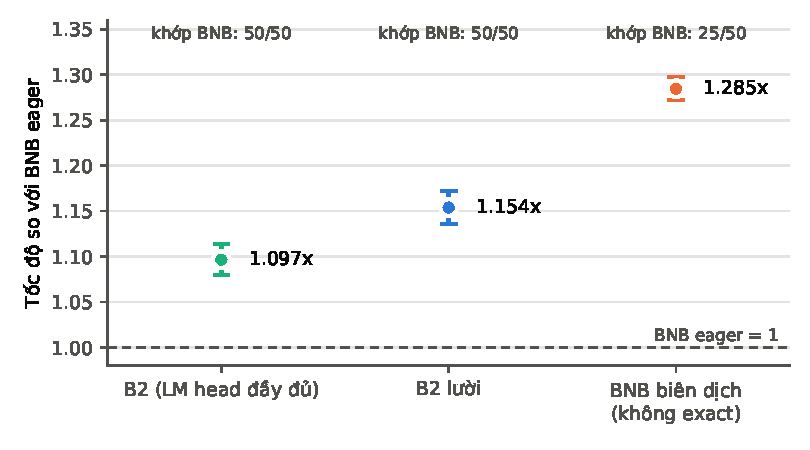
\includegraphics[width=0.78\textwidth]{images/tr_methods_heldout2.pdf}
\caption{Tốc độ so với BNB eager trên held-out GSM8K $400$--$449$ (50 prompt; điểm là trung bình nhân, thanh là khoảng tin cậy $95\%$). Dòng trên cùng ghi số prompt có token khớp BNB eager. BNB biên dịch nhanh hơn nhưng chỉ khớp $25/50$.}\label{fig:methods}
\end{figure}

\subsection{So sánh với baseline biên dịch}\label{sec:compiled}
Một vòng decode BNB với \code{StaticCache} và \code{torch.compile} (mode \code{reduce-overhead}) nhanh hơn BNB eager \ci{1.285}{1.272}{1.297}$\times$ trên held-out $400$--$449$, đo cạnh nhau cùng lượt chạy. Tuy nhiên token của nó chỉ khớp eager ở $25/50$ prompt, tức không phải tham chiếu bitwise. B2 lười đạt $0.907\times$ [$0.893$, $0.920$] tốc độ của nó và chậm hơn ở $49/50$ prompt (trên dev: $0.82\times$, $12$ prompt). Vì vậy luận điểm đúng của B2 là ``exact so với BNB eager, nhanh hơn eager khoảng $1.1$--$1.25\times$'', không phải ``nhanh hơn baseline mạnh''. Chưa thử kết hợp compile với giải mã suy đoán; nó sẽ đổi số học và đòi hỏi định nghĩa lại tham chiếu.

\subsection{Ngữ cảnh dài và các mô hình khác}
\begin{figure}[t]
\centering
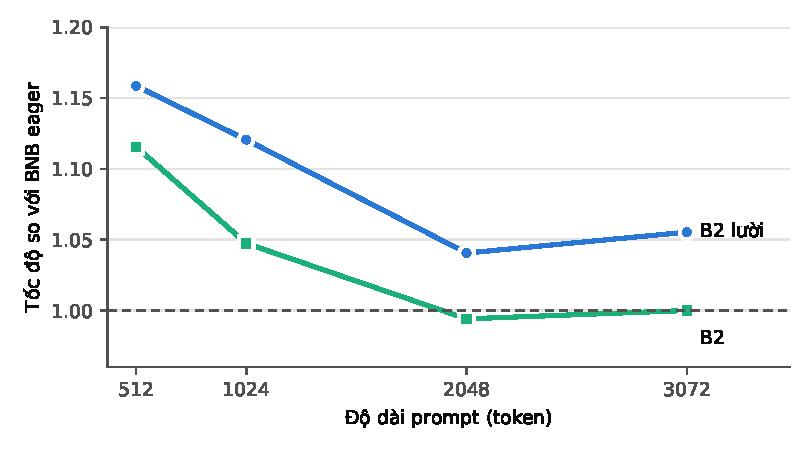
\includegraphics[width=0.78\textwidth]{images/tr_context_length.pdf}
\caption{Tốc độ so với BNB eager theo độ dài prompt (3 prompt dev mỗi độ dài, tóm tắt nhiều bài CNN/DM ghép lại).}\label{fig:context}
\end{figure}
Token và KV khớp ở mọi độ dài tới $3071$ token, nhưng tốc độ giảm (Hình~\ref{fig:context}): B2 lười còn $1.04$--$1.06\times$ ở $2048$--$3072$ token. Chi phí một forward gần như không đổi theo độ dài (wall: BNB $M{=}1$ $23.2\to23.5$ ms), nên nguyên nhân đã đo là acceptance thấp trên tác vụ tóm tắt ($0.24$--$0.29$ ở $3072$ so với $0.32$--$0.64$ ở $512$) và prefill chung ($1.1$ s ở $3072$ token) làm loãng tỷ lệ; chưa có prompt dài mà acceptance cao để tách hoàn toàn hai yếu tố. Trên Qwen2.5-0.5B và 1.5B (10 prompt dev) B2 lười đạt $1.243\times$ và $1.163\times$, token và KV khớp $10/10$.

\subsection{Bộ nhớ}
Ở cùng dung lượng cache tĩnh, đỉnh bộ nhớ cấp phát của B2 chỉ lớn hơn BNB eager $0.07$~MiB ($2007.90$ so với $2007.97$ MiB ở prompt $75$ token; $2994.61$ so với $2994.68$ MiB ở $3071$ token); đỉnh dự trữ và bộ nhớ thiết bị dùng giống hệt nhau, và không có mô hình draft. Mỗi phương pháp chạy trong một tiến trình riêng, đo ở lượt thứ hai.

\subsection{Phân tích chi phí}
Một forward khối $M{=}3$ tốn $37.1$ ms, gấp $1.65$ lần một bước $M{=}1$ ($22.5$ ms), nên block chỉ có lợi khi sinh trên $1.65$ token mỗi chu kỳ (acceptance khoảng $33\%$ với hai đề xuất); trung bình $1.86$ token mỗi chu kỳ khối và $73\%$ chu kỳ phải quay về bước gốc, khớp với mức tăng tốc khoảng $12$--$15\%$. LM head bf16 tốn khoảng $3.3$ ms mỗi hàng và là phần lớn của chênh lệch GPU, nên chiếu lười có ích. Cả hai loại forward bị giới hạn bởi CPU khởi chạy kernel ($84\%$ thời gian một bước $M{=}1$ là enqueue CPU), điều này cũng giải thích vì sao baseline biên dịch (giảm overhead CPU) nhanh hơn.

\subsection{Thăm dò: chụp CUDA graph (ước lượng, chưa cài đặt)}
Chúng tôi chụp thô một bước decode $M{=}1$ của mô hình bitsandbytes eager với \code{StaticCache} bằng CUDA graph (không \code{torch.compile}, cùng các kernel): chụp được, logits bằng từng bit ở $64/64$ bước, và chi phí giảm từ $22.5$ xuống $17.3$ ms mỗi bước ($1.30\times$). Khối chuẩn ba hàng (không exact) tốn $27.4$ ms ở chế độ eager và $23.9$ ms trong graph. Ghép với mô phỏng đã hiệu chỉnh, một vòng B2 chạy phần thân decoder trong graph (các phép từng hàng nằm trong graph nên không còn tốn CPU) với LM head lười chạy ngoài graph cho tốc độ ước lượng $1.36$--$1.48\times$ so với eager, nhưng chỉ $1.04$--$1.14\times$ so với một baseline graph exact. Đây là dự đoán từ mô hình chi phí (chi phí decoder ba hàng trong graph $21.7$--$24.0$ ms ước từ số đo kernel), chưa được cài đặt, nên không phải kết quả đã đo của B2.

\section{Các kết quả bất lợi và hướng không hiệu quả}\label{sec:negative}
\begin{itemize}[nosep]
\item \textbf{Chọn n-gram.} Quét độ dài n-gram $2$--$5$ chênh dưới $2\%$ và nằm trong nhiễu đo. Bảy chính sách chọn draft (lọc đề xuất yếu, bỏ phiếu giữa các lần khớp, ngưỡng lặp) đều khớp BNB; lọc đề xuất yếu không nhanh hơn dù giảm gần một nửa số khối, và bỏ phiếu so với chính sách gốc cho tỷ số \ci{1.002}{0.998}{1.007} trên $80$ prompt dev chưa dùng để chọn. Giữ chính sách gốc.
\item \textbf{Giảm chi phí CPU.} Gọi thẳng kernel Triton đã biên dịch cho kết quả bằng nhau từng bit nhưng không nhanh hơn ($7.22$ so với $7.59$ ms cho $252$ phép chiếu); các điểm nóng còn lại là chuỗi phép PyTorch nhỏ ở RMSNorm và attention từng hàng, không thể giảm mà không đổi tập kernel.
\item \textbf{Khối lớn hơn.} Mô phỏng (chạy PLD trên chuỗi tham chiếu đã ghi, chi phí mỗi hàng hiệu chỉnh khớp $K{=}2$ đo được) dự đoán $K{=}3,4$ thay đổi từ $-1\%$ đến $+2.6\%$ so với $K{=}2$ (tới $+4.1\%$ nếu chi phí mỗi hàng giảm một nửa); không đáng viết kernel mới. Đây là dự đoán từ mô hình tuyến tính, chưa kiểm bằng thực nghiệm.
\item \textbf{Quay về bước gốc.} Quay về $M{=}1$ khi không có đề xuất đưa tốc độ từ $0.91$--$0.97\times$ lên $1.06$--$1.15\times$ trên các cohort dev nhỏ; đây là thay đổi đóng góp lớn nhất.
\end{itemize}

\section{Giới hạn và mối đe dọa tính hợp lệ}
\begin{itemize}[nosep]
\item \textbf{Phạm vi.} Một GPU và bộ công cụ, chủ yếu một họ mô hình (Qwen2), một backend lượng tử hóa (bitsandbytes), batch 1, greedy, $k{=}2$. Kết quả không áp dụng được cho lấy mẫu, batch lớn hay các lược đồ lượng tử hóa khác.
\item \textbf{Chứng minh.} Tính exact dựa trên bằng chứng hữu hạn. Còn mở: bằng kernel bitsandbytes trên mọi đầu vào, độc lập của dispatch PyTorch với số hàng, độ ổn định qua phiên bản Triton/ptxas/CUDA và GPU, kiểm ở mức PTX.
\item \textbf{Chọn cấu hình.} Cấu hình được chọn trên dev; hai cohort held-out không dùng để chọn, nhưng cohort $400$--$449$ được dùng để đánh giá riêng biến thể B2 lười đã cố định trước đó, và cohort $300$--$349$ chỉ đánh giá biến thể LM head đầy đủ.
\item \textbf{Khoảng tin cậy.} Chỉ phản ánh biến thiên giữa các prompt đã chọn, không phải toàn bộ workload. Tốc độ tuyệt đối phụ thuộc cohort ($1.23\times$ ở HumanEval $0$--$19$ nhưng $1.31\times$ ở $20$--$49$).
\item \textbf{Baseline.} Tốc độ chỉ so với BNB eager; baseline biên dịch nhanh hơn nhưng không exact.
\end{itemize}

\section{Tóm tắt chương}
Với Qwen2.5-3B NF4 trên một GPU tiêu dùng, B2 tái tạo đúng từng token và KV của greedy bitsandbytes, không dùng thêm bộ nhớ đáng kể và nhanh hơn eager khoảng $12$--$15\%$ trên hai cohort held-out; mức tăng khiêm tốn và bị giới hạn bởi chi phí khởi chạy CPU và acceptance của PLD. Giá trị chính nằm ở tính exact và quy trình bằng chứng chứ không ở tốc độ. Hướng tiếp theo gồm kiểm ở mức PTX và trên GPU/phiên bản Triton khác, mở rộng sang backend lượng tử hóa và họ mô hình khác, và chứng minh hợp đồng toán tử.

Mã, bằng chứng thô và kịch bản tái lập nằm trong kho mã (thư mục \texttt{experiments}).
